\documentclass[12pt]{article}

\usepackage{url}
\usepackage{fullpage}
\usepackage{enumerate,amsmath,amsthm}
\usepackage{amssymb,amsfonts}
\usepackage{mathtools}
\usepackage{setspace}
\usepackage{dsfont}
\usepackage[margin=.9in]{geometry}

\onehalfspacing

\usepackage[normalem]{ulem}
\setlength{\parindent}{0pt}
\setlength{\parskip}{0.5em}%

\begin{document}

\begin{center}
{\Large \textsc{CS 171 Project Proposal}}

\bigskip

{\large Jacob Kim, George Qi, and Lawrence Kim}

\smallskip

\end{center}

\subsection*{Background and Motivation}
\vspace{-3mm}
{\it Discuss your motivations and reasons for choosing this project, especially any background or research interests that may have influenced your decision.}

The United States housing market is one of the most relevant and impactful markets in many of our households. In particular, the housing bubble in 2006 and 2007 that strongly contributed to the 2007-2009 recession was one of the most significant economic events thus far in our lifetime. That being said, I believe very few people, especially at our age, have a strong understanding of the housing market and the discrepancies in simple metrics, even price. Although we may have general views (i.e. New York or California tend to be expensive, while rural areas remain cheap), we thought it would be interesting to take a closer look at the housing market and generate an interesting and effective way to view the big picture in a single location.

\subsection*{Project Objectives}
\vspace{-3mm}
{\it Provide the primary questions you are trying to answer with your visualization. What would you like to learn and accomplish? List the benefits.}

Primary questions include:
\vspace{-3mm}
\begin{enumerate}
\item Which geographic areas tend to be more expensive?
\item Aside from inflation, when did housing prices tend to decrease/increase? Why is this the case?
\item Which features tend to affect price most heavily?
\item If we made a histogram on the house prices, what kind of distribution would it follow? How heavily is it skewed, if at all? Does this vary by region?
\end{enumerate}
\vspace{-1mm}

Other questions that we would like to think about incorporating into another visualization beyond just the analysis of the housing market would include linking this data with data on the US economy. It is intuitive that when the economy is growing, so should the average house price, but the real question is: to what degree? Perhaps although the country's GDP is rapidly growing, certain states or cities have yet to see their house prices increase very much. Or perhaps there are certain odd time periods that we can point out from our trends that can be linked to an economic event, such as a law passed or whatnot. Bringing in other datasets would certainly be very interesting.

As for benefits, we believe our project would solve a common problem that we've noticed. When observing discrepancies in house prices, we have come across little to no visualization tools. We generally come across raw numbers for certain states, cities, etc., but in this form of presentation, it can be difficult to draw conclusions about the housing market (especially regional ones). This is exactly where visualization comes in and works best. Our project would enable newer, less informed people to learn a great deal of information in a limited amount of time. Its interactive nature would also attractive interest from people who would have otherwise been less interested. 

Bringing in the additional economic data sets would also give the users an even better understanding of how the economy as a whole affects and is affected by the housing market. 

\subsection*{Data}
\vspace{-3mm}
{\it From where and how are you collecting your data? If appropriate, provide a link to your data sources.}

We are collecting our data from \url{http://www.zillow.com/research/data}, which has been provided in the Section 7 notes. The website has their data available in a multitude of CSV files, which we will download and extract information from in order to collect the housing data that we need.

\subsection*{Data Processing}
\vspace{-3mm}
{\it Do you expect to do substantial data cleanup? What quantities do you plan to derive from your data? How will data processing be implemented?}

Since all data will be present in separate CSV files, a substantial amount of our data cleanup will involve combining all the data from these separate CSV files such that we can properly use them for data visualization. 
From the data, we have to contain prices for all types of houses from 1 bedroom houses all the way up to 5+ bedroom houses, and other potential filtering factors, such as whether a house is ``top tier'' or ``bottom tier''. Since we will most likely be utilizing cities to show housing prices, we will want to obtain data that corresponds to the cities. In addition, since we will eventually want to group the cities by the state they are in, we will want all data of such cities to be contained within an object representing the states.

After data processing is done, we will want convert to a JSON file to contain an object called states that contains an array of objects called cities for each state. Within each of these cities objects, there will be an array of objects called months, that will contain information for each month. Within that month object, there will be average prices for houses, based on the characteristics (such as number of bedrooms or what tier the house is in). To facilitate processing when we actually implement the visualization, we could also just have such average prices be present within the state objects themselves, such that we don't have to average over all cities within a state.

An alternative is just to merge the CSV files and then create a data frame.

\subsection*{Visualization}
\vspace{-3mm}
{\it How will you display your data? Provide some general ideas that you have for the visualization design. Include sketches of your design.}

We have at least two ideas for the visualization template: the sketches can be found below.

\begin{center}
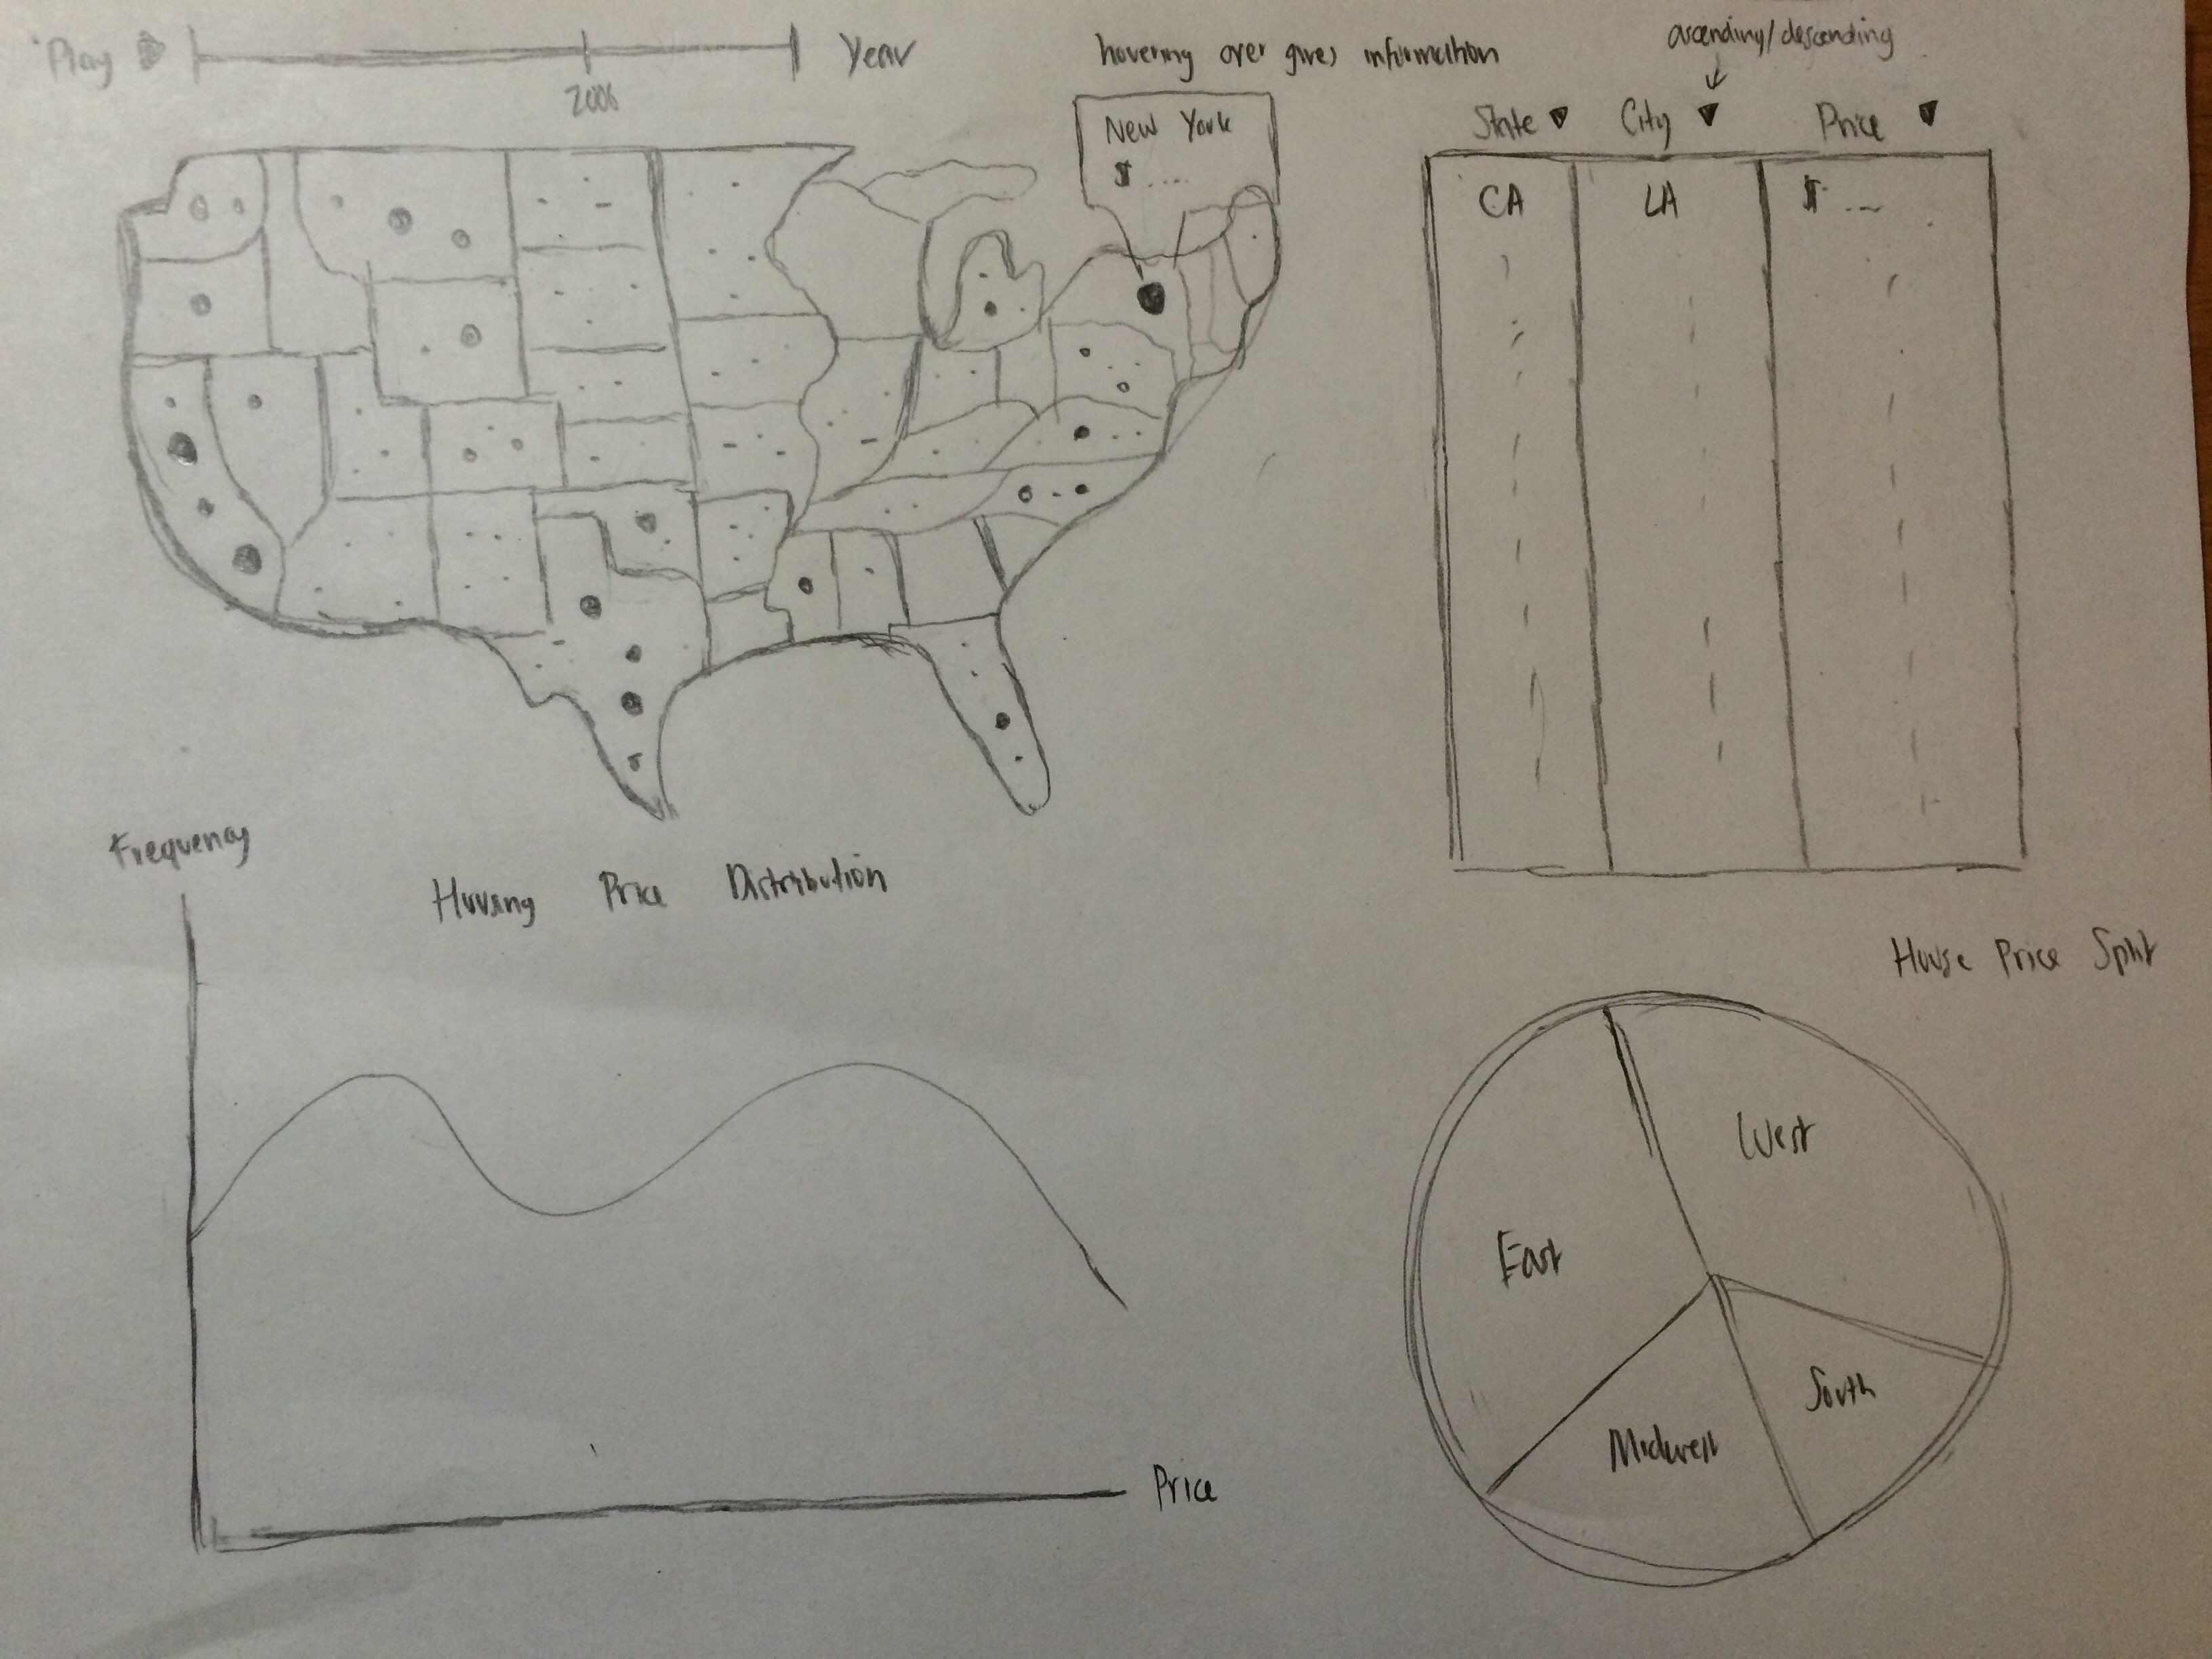
\includegraphics[scale=0.13]{pic1.jpg}
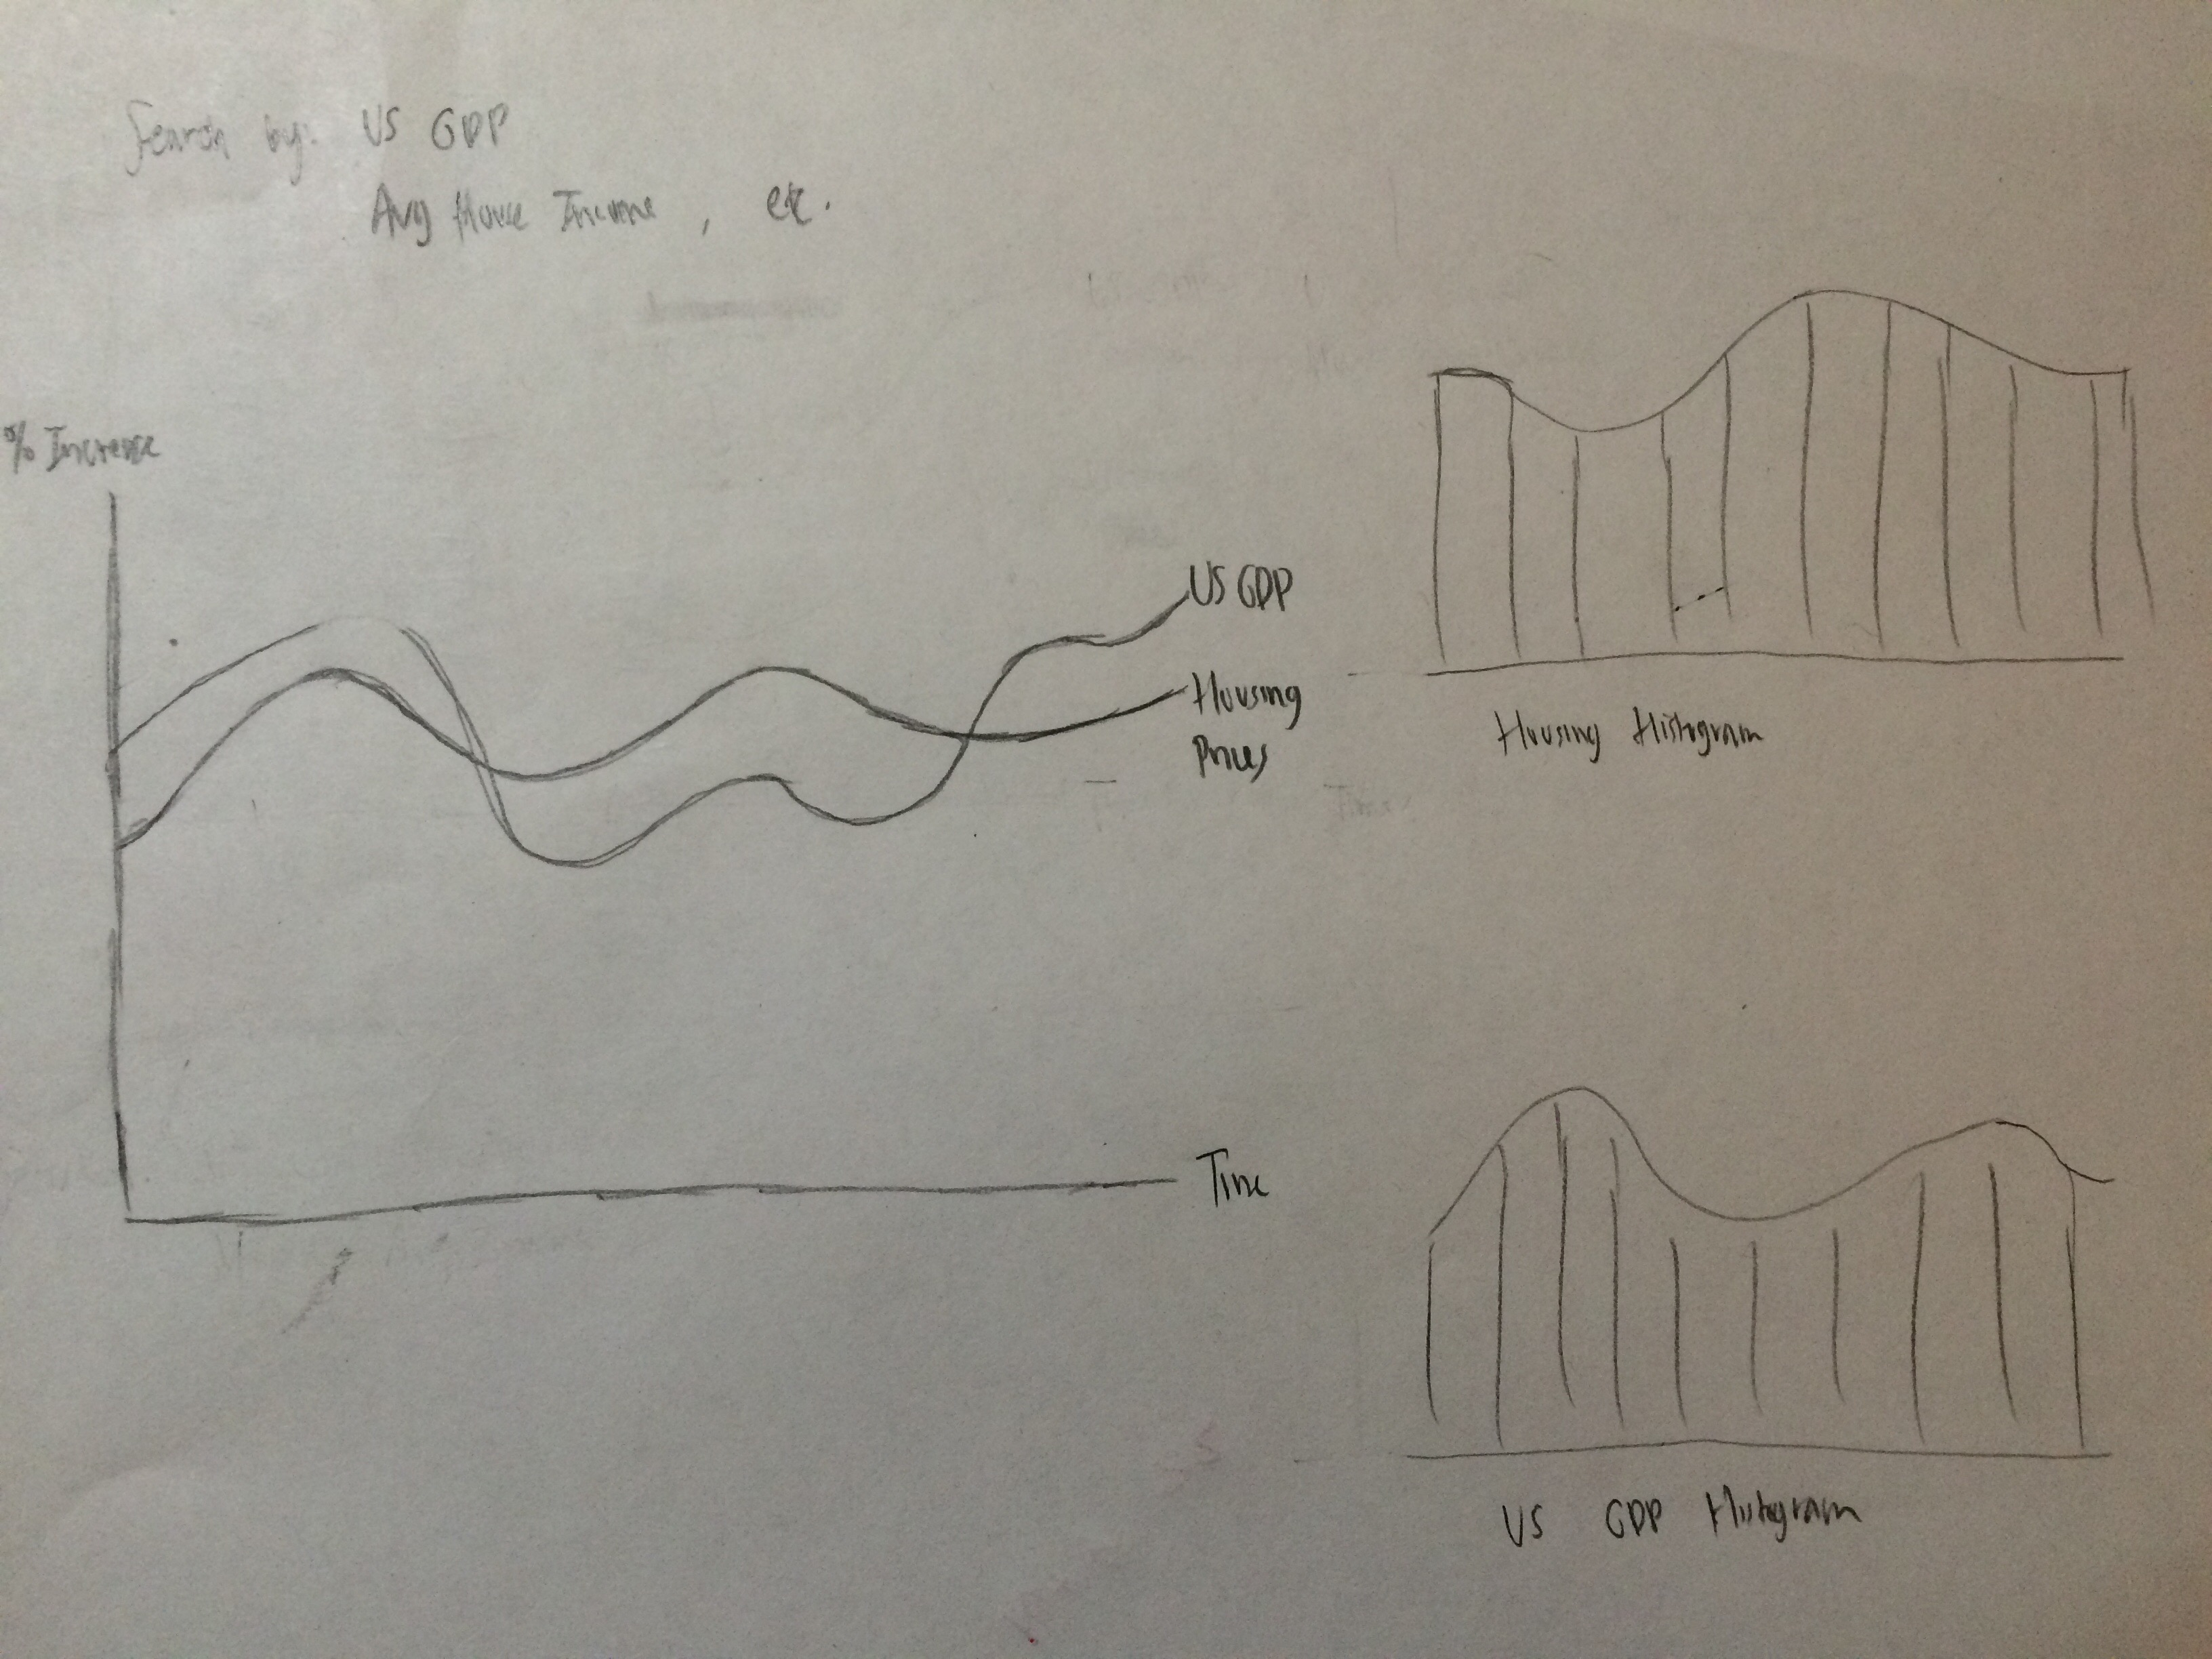
\includegraphics[scale=0.13]{pic2.jpg}
\end{center}

First, there will be a map of the United States. For each city, there will be a node for representation. The size of that node will increase/decrease based on how high the average prices are. But since some cities will have much higher prices than others (such as cities in the slums), we'll scale by having a maximum size and a minimum size, such that even the lowest priced cities can have visibility. In addition, by hovering over a node, it should display general information, such as the average price of houses, and the name of the city. We would also implement a time-slider mechanism such that we could filter through different times.

In addition to the map, there could be a table that ranks the cities based on prices. We could filter through these rankings based on the characteristics and month. If we were able to maintain the number of houses within each city, we could also find the aggregate housing prices for each location. Upon knowing aggregate housing prices, there could also be a pie chart, that shows the amount of housing price share that each region contains.

Below the map, there would also be a histogram showing the distribution of house prices for that time period so that we can have a holistic, visual view of how frequently some prices occur over others. To prevent distortion, we would weight this by the number of houses in each city, because it would certainly be unfair to weight New York the same as Iowa.

Finally, in the corner of the visualization, we would have a pie chart showing how dominant certain regions are within the housing market.

Second, we could incorporate another data source (such as economic GDP/annual income data) that would help create links between the housing market and the general economy as a whole. That is, given the growth (or lack thereof) of the economy, how does the housing market respond? There would be a general graph documenting the changes in the economy versus the changes in the housing market, as well as distributions of both on the right hand side, that would lend a closer look.

\subsection*{Must-Have Features}
\vspace{-3mm}
{\it These are features without which you would consider your project to be a failure.}

\begin{enumerate}
\item Map of USA showing the cities marked by circles
\item Size of circle can represent price
\item Time-slider that shows how prices change over time
\item Filter by type of home (1 bedroom, 2 bedroom, house, etc.)
\item Include at table ranking the cities by prices
\end{enumerate}

\subsection*{Optional Features}
\vspace{-3mm} 
{\it Those features which you consider would be nice to have, but not critical.}

\begin{enumerate}
\item A play button to show an animation of house housing prices have changed over time
\item Add other metrics in addition to average prices
\item Search bar
\item Filter cities by a set price range
\item Line graph that shows a line graph of price vs. time for a selected city
\item Data aggregation for states/regions
\item Histogram of housing prices
\item Add in other data sets
\end{enumerate}

\subsection*{Project Schedule}
\vspace{-3mm}
{\it Make sure that you plan your work so that you can avoid a big rush right before the final project deadline, and delegate different modules and responsibilities among your team members. Write this in terms of weekly deadlines}

\underline{\textbf{Week 1 (April 4-10)}}
\begin{enumerate}
\item Pick which data sets to use from Zillow
\item Transform data (merge all the CSVs into one and then convert to JSON)
\item Finalize sketches
\item Delegate tasks and responsibilities
\item Start implementation 
\end{enumerate}

\underline{\textbf{Week 2 (April 11-17)}}
\begin{enumerate}
\item Implement map of US with prices represented as circles
\item Implement table of cities
\end{enumerate}

\underline{\textbf{Week 3 (April 18-24)}}
\begin{enumerate}
\item Create time slider
\item Create filter by home type option
\end{enumerate}

\underline{\textbf{Week 4 (April 25-May 1)}}
\begin{enumerate}
\item Consider other optional features and implement them
(Search bar, line graph, different views, play button)
\end{enumerate}

\underline{\textbf{Week 5 (May 2-5)}}
\begin{enumerate}
\item Add in any last minute optional features
\item Improve design
\item Request feedback and make appropriate changes based on feedback
\item FINALLY: Submit
\end{enumerate}

\end{document}

